\documentclass{article}
\newsavebox{\oldepsilon}
\savebox{\oldepsilon}{\ensuremath{\epsilon}}
\usepackage[minionint,mathlf,textlf]{MinionPro} % To gussy up a bit
\renewcommand*{\epsilon}{\usebox{\oldepsilon}}
\usepackage[margin=1in]{geometry}
\usepackage{graphicx} % For .eps inclusion
%\usepackage{indentfirst} % Controls indentation
\usepackage[compact]{titlesec} % For regulating spacing before section titles
\usepackage{adjustbox} % For vertically-aligned side-by-side minipages
\usepackage{array, amsmath, mathrsfs, mhchem}
\usepackage{hyper ref}
\usepackage{courier, subcaption}
\usepackage{multirow, color}
\usepackage[autolinebreaks,framed,numbered]{mcode}

\usepackage{float}
\restylefloat{table}
\newcommand{\Lapl}{\mathcal{L}}

\pagenumbering{gobble} 
\setlength\parindent{0 cm}
\renewcommand{\arraystretch}{1.2}
\begin{document}
\large

\section*{Recap of the two-step negative autorepression system}

\begin{itemize}
\item Last time, we began our study of negative autoregulation using control theory.
\item Intuition suggested that this system could be used to maintain the concentration of a repressor at a desired value, dampening any fluctuations that might occur e.g. due to varying levels of transcriptional activation.
\item I warned you, however, that negative autoregulation might not always work as planned. In some cases it leads to chronic oscillations and/or amplifies small deviations from the desired value.
\item We focused our attention on a transcriptional repressor that regulates its own production with negative feedback that is proportional to the error (that is, to the deviation of the repressor's concentration from its desired value, which we assumed for simplicity to be 0).
\item This system can be described by the block diagram
\begin{center}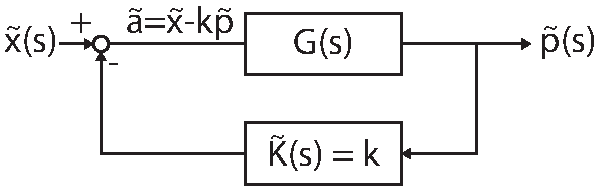
\includegraphics[width=0.5 \textwidth]{autorepression_twostep.pdf}\end{center}

\item By considering the topology of our control loop, we determined the closed loop transfer function $\tilde{p}/\tilde{x}$ can be written as:

\[ \tilde{p}(s) = G(s) \tilde{a}(s) \implies \frac{\tilde{p}(s)}{\tilde{x}(s)} = \frac{G(s)}{1 + kG(s)} \]


\item Our motivation for the proportionality assumption was that if the repressor binds its own promoter hyperbolically, and the error term is small, then the slope of the repressor's binding curve is approximately linear with a slope we called $k$ (the repressor's ``gain").

\item To find a form for the open loop transfer function $G(s)$, we had to specify some particulars about the \textit{plant} -- that is, the LTI system relating the net repressor mRNA expression ($a(t)$) to the concentration of the repressor protein. We did this using a pair of differential equations:
\begin{eqnarray*}
\frac{dm}{dt} & = & c_m a(t) - \gamma_m m(t)\\
\frac{dp}{dt} & = & c_p m(t) - \gamma_p p(t)
\end{eqnarray*}

\item By taking the Laplace transform of these, and assuming that the initial concentrations of protein and mRNA were zero for simplicity, we found the open loop transfer function:

\[ G(s) = \frac{\tilde{p}(s)}{\tilde{a}(s)} = \frac{c_p c_m}{\left( s + \gamma_p \right)\left( s + \gamma_m \right)} \]

\item Na\"{i}vely, it appeared that choosing a large value of $k$ would ensure that the error in the system's output, i.e. $\tilde{p}(s)$-0, stayed small. However, I warned that increasing $k$ might make the system unstable.

\item We discussed how $\tilde{p}(s)$ (for an appropriate choice of $\tilde{x}(s)$) could be rewritten using partial fraction decomposition into a sum containing terms of the form $\frac{z_i}{s-\alpha_i}$, where the $\alpha_i$ were the \textit{poles} of the closed loop transfer function (multiplied by $\tilde{x}(s)$).

\item This implied that $p(t)$ would be equal to a sum of terms of the form $e^{-\alpha_i t}$. In other words, if a pole $\alpha_i$ of the closed loop transfer function had a positive real part, then that term would grow indefinitely with time, and so $p(t)$ would diverge.

\item We therefore wanted to know whether increasing $k$ could make one or more of the $\alpha_i$ have a positive real part. If so, choosing a large gain would cause our system to become unstable.

\end{itemize}

\section*{Continuation of the discussion of the Nyquist stability criterion}

\begin{itemize}

\item Where are the poles of our closed loop transfer function? The numerator, $G(s)$, contributes two poles: $s=-\gamma_m$ and $s=-\gamma_p$. Neither of these poles have positive real part. That means that if the closed loop transfer function has any poles with positive real part, they must be the roots of the denominator, $1+kG(s)$.

\item We needed a method to determine whether there were any roots of $1+kG(s)$ in the right half of the complex plane. We began to introduce the Nyquist stability criterion for this purpose.

\item The Nyquist stability criterion relates the number or roots and poles of a function inside the Nyquist contour to the shape of its Nyquist plot. The Nyquist plot of $1+kG(s)$ is drawn by plugging every point $s$ on the Nyquist contour into $1+kG(s)$.

\item The Nyquist contour runs up the imaginary axis, then back to $-i\infty$ through the right half plane along a semicircular arc of radius infinity.

\item The number of times the Nyquist plot of $1+kG(s)$ encircles the origin going clockwise ($N$) is equal to the number of zeros of $1+kG(s)$ inside the Nyquist contour ($Z$) minus the number of poles of $1+kG(s)$ inside the Nyquist contour ($P$).

\item The parameter $k$ is not fixed in our model, so we can't easily draw a Nyquist plot of $1+kG(s)$. However, a handy feature of the way the plot shifts and scales is that $N$ is also equal to the number of times the Nyquist plot of $G(s)$ encircles the point $-1/k$ going clockwise. This allows us to draw one Nyquist plot (of $G(s)$) and easily consider different values of $k$.

\item In order to find $Z$, we need both $N$ and $P$. $N$ we determine from the Nyquist plot; $Z$ we can get by examination of $1+kG(s)$. The poles of $1+kG(s)$ must be the same as the poles of $G(s)$. (If not convinced, try combining these terms under a common denominator.)

\item We already know that the poles of $G(s)$ are $s=-\gamma_m$ and $s=-\gamma_p$, neither of which have positive real part. Therefore, $Z=0$.

\item To find $N$, we can draw the Nyquist plot if the $c_i$ and $\gamma_i$ are fixed.  This can be done in MATLAB using \mcode{tf()} to define the transfer function $G(s)$ and \mcode{nyquist()} to draw the plot. [Draw what the result looks like.]

\item To convince ourselves that this is not a property of our choice of parameters, we can make a graphical argument. In order for $-1/k$ to be enclosed, the Nyquist plot would have to cross the real axis at least once at a negative real value. (This is not sufficient, but it is necessary). Now we will attempt to determine whether it does so by looking at $G(s)$ for points $s$ on the Nyquist contour.

\item On the semicircular arc, $|s|$ is infinite. Clearly $G(s)=0$ for all points on the semicircular arc.

\item To find where $G(s)$ maps the points on the imaginary axis, i.e., what is $G(i\omega)$ for $\omega \in (-\infty, \infty)$, we plug in $s=i\omega$ and rearrange to get a real denominator:

\begin{eqnarray*}
G(i \omega) & = &  \frac{c_p c_m}{\left( i\omega + \gamma_p \right)\left( i\omega + \gamma_m \right)} \cdot \frac{\left(- i\omega + \gamma_p \right)\left( - i\omega + \gamma_m \right)}{\left(- i\omega + \gamma_p \right)\left(- i\omega + \gamma_m \right)}\\
& = & \frac{c_p c_m \left[  - \omega^2 + \gamma_p \gamma_m -i \omega \left(\gamma_p + \gamma_m \right) \right]}{\left( \omega^2 + \gamma_p^2 \right)\left( \omega^2 + \gamma_m^2 \right)}
\end{eqnarray*}

\item This implies that the contour crosses the imaginary axis at a positive real value of $w$ (as well as at $w=0+0i$). In other words, no points on the negative real axis are ever enclosed, and it does not matter how large we choose $k$.
\end{itemize}


\section*{Comparison to a three-step pathway}

\begin{center}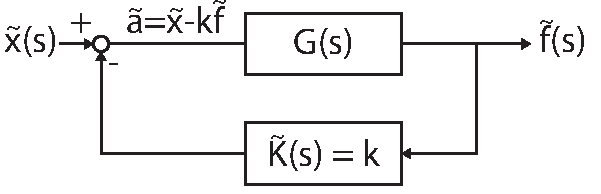
\includegraphics[width=0.5 \textwidth]{autorepression_threestep.pdf}\end{center}

\begin{itemize}

\item As we alluded to last time, something surprising happens when we make our ``plant" only slightly more complicated by adding a third step to the negative autoregulation.

\item Suppose the protein $p$ produces a chemical ($f$) that represses expression of the gene:

\begin{eqnarray*}
\frac{dm}{dt} & = & c_m a(t) - \gamma_m m(t)\\
\frac{dp}{dt} & = & c_p m(t) - \gamma_p p(t)\\
\frac{df}{dt} & = & c_f p(t) - \gamma_f f(t)
\end{eqnarray*}

\item We now consider the system's output to be $f(t)$, not $p(t)$. Similarly, $a(t) = x(t) - k f(t)$.

\item Performing the Laplace transforms and algebraic rearrangements as above, we find that when $m(0)=p(0)=f(0)$:

\[ G(s) = \frac{c_p c_m c_f}{\left( s + \gamma_p \right)\left( s + \gamma_m \right)\left( s + \gamma_f \right)} \]

\item Analysis of this system proceeds exactly as before. The closed loop transfer function $G(s)/(1+kG(s))$ has poles with positive real part only when the denominator, $1+kG(s)$, has roots with positive real part. The denominator has no poles with positive real part. Therefore, by the Nyquist stability criterion, $Z>0$ if and only if the Nyquist plot of $G(s)$ encloses the point $-1/k$.

\item As before, $G(s)=0$ on the semi-circular arc of the Nyquist contour, so we can draw the Nyquist plot by calculating $G(i \omega)$ for $\omega \in (-\infty, \infty)$.

\item Although this looks quite similar to the above, we will find that the system's behavior has changed qualitatively:
\begin{eqnarray*}
G(i \omega) & = &  \frac{c_p c_m c_f}{\left( i\omega + \gamma_p \right)\left( i\omega + \gamma_m \right)\left( i\omega + \gamma_f \right)} \cdot \frac{\left(- i\omega + \gamma_p \right)\left( - i\omega + \gamma_m \right)\left( -i\omega + \gamma_f \right)}{\left(- i\omega + \gamma_p \right)\left(- i\omega + \gamma_m \right)\left( -i\omega + \gamma_f \right)}\\
& = & \frac{c_p c_m c_f \left[ \gamma_p \gamma_m \gamma_f - \omega^2 \left(\gamma_p + \gamma_m + \gamma_f \right) + i \omega \left( \omega^2 - \left[ \gamma_p \gamma_m + \gamma_p \gamma_f + \gamma_m \gamma_f \right] \right) \right]}{\left( \omega^2 + \gamma_p^2 \right)\left( \omega^2 + \gamma_m^2 \right)\left( \omega^2 + \gamma_f^2 \right)}
\end{eqnarray*}

\item Now the plot crosses the real axis in two more places ($\omega \propto \pm \sqrt{ \gamma_p \gamma_m + \gamma_p \gamma_f + \gamma_m \gamma_f}$), and the real part of $G(i\omega)$ at those crossings is the same:

\[ c_p c_m c_f \left[ \gamma_p \gamma_m \gamma_f - \left( \gamma_p \gamma_m + \gamma_p \gamma_f + \gamma_m \gamma_f \right) \left(\gamma_p + \gamma_m + \gamma_f \right) \right] < 0  \]

\item The full Nyquist plot confirms our suspicion that some points on the negative real axis have been enclosed by the contour. If $-1/k$ falls within that range (i.e. if $k$ is sufficiently large),  the system becomes unstable. The gain will need to be kept below a threshold determined by the parameters above in order to prevent instabilty.

\item The more steps are included in a process, the easier it is for that process to become unstable; in a system with five components, the threshold gain $k$ would be even lower.

\item In these toy models, instability would imply that the system diverged. However, in biological systems, limited resources and the requirement that concentrations be non-negative ensures that a system will not really diverge. Instead, the system will likely either saturate or oscillate depending on the circumstances.

\item Long pathways are not the only sources of instability. The second problem on your fifth problem set will walk you through applying the Nyquist stability criterion in the case where we have a two-step system (i.e. we model just the repressor's mRNA and protein), but with a time delay between mRNA production and translation. To keep things simple, instead of solving the general case, you'll ultimately create a Nyquist plot for a particular set of parameter values. Every major step of the derivation is covered.

\item For now, however, we turn to another source of instability in negative autoregulation systems: non-linearity.
\end{itemize}

\section*{Goodwin oscillator}

\begin{itemize}
\item In the three-step pathway we just studied, when $k$ was too large, any small deviation of the input $x(t)$ from zero would cause the system to diverge. (If $x(t)=0$ for all time, then the mRNA, protein, and compound $f$ are never produced and $p(t)=0$ forever.) This manifests as oscillations that grow indefinitely in magnitude: not a very realistic outcome for a biological system (where concentrations do not fall below zero or rise indefinitel).

\item Through much of the course we have emphasized that biological systems are, for better or worse, slave to non-linear effects like hyperbolic binding, Michaelis-Menten kinetics, cooperativity, zero-order ultrasensitivity, and the like.

\item Since negative autoregulation is pervasive in biological systems, we might ask whether we have ``lost anything" by ignoring non-linearity. Might it be the case that these nonlinear terms foster stability in the system? Impede it?

\item We will see that a modified version of the three-step model studied earlier, assuming cooperativity in repressor binding, causes one of the behaviors commonly observed in natural negative autoregulation systems: stable oscillations.

\item We model an autoregulatory system where an mRNA $m$ begets a protein $p$ which begets a chemical compound $c$. The compound $f$ then acts cooperatively to inhibit expression of the mRNA (perhaps, by binding to a multimeric repressor to activate it).

\begin{eqnarray*}
\frac{dm}{dt}& = &\frac{a_1 K}{K + f^n} - b_1 m\\
\frac{dp}{dt} &= &a_2 m - b_2p\\
\frac{df}{dt} &= &a_3 p - b_3f
\end{eqnarray*}

\item We have a model with eight parameters. I will claim that four are superfluous, and that we can rewrite these equations in the form:

\begin{eqnarray*}
\frac{dz_1}{dt} &= &\frac{1}{1 + z_3^n} - c_1 z_1\\
\frac{dz_2}{dt} &= &z_1 - c_2 z_2\\
\frac{dz_3}{dt} &= &z_2 -c_3 z_3
\end{eqnarray*}

\item To achieve this, we will rescale all variables -- time and each concentration -- by an unknown constant. After substituting the scaled variables into our original equation, we can determine what the scaling factors should be.

\item We define scaling factors $w$ and $h_i$ such that $\tau = wt$, $z_1 = h_1 m$, $z_2 = h_2 p$, and $z_3 = h_3 f$. The first equation simplifies to:
\begin{eqnarray*}
\frac{dm}{dt} &=&\frac{w}{h_1} \frac{dz_1}{d\tau} = \left( a_1 \right) \frac{1}{1 + (\frac{z_3}{h_3 \sqrt[n]{K}})^n} - \left( \frac{b_1}{h_1} \right) z_1\\
\frac{dz_1}{d\tau}& =& \left( \frac{a_1h_1}{w} \right) \frac{1}{1 + (\frac{z_3}{h_3 \sqrt[n]{K}})^n} - \left( \frac{b_1}{w} \right) z_1
\end{eqnarray*}
The second equation to:
\begin{eqnarray*}
\frac{dp}{dt}& = &\frac{w}{h_2} \frac{dz_2}{d\tau} = \left( \frac{a_2}{h_1} \right) z_1 -  \left( \frac{b_2}{h_2} \right) z_2\\
\frac{dz_2}{d\tau}& = &\left( \frac{a_2 h_2}{wh_1} \right) z_1 -  \left( \frac{b_2}{w} \right) z_2
\end{eqnarray*}
And finally, by analogy, the third equation:
\begin{eqnarray*}
\frac{dz_3}{d\tau} = \left( \frac{a_3 h_3}{wh_2} \right) z_2 -  \left( \frac{b_3}{w} \right) z_3
\end{eqnarray*}

\item In order for these three equations to match the simplified version I proposed, we find that we need:

\[ h_3 = \frac{1}{\sqrt[n]{K}} \hspace{2 cm} \frac{a_1h_1}{w} = 1 \hspace{2 cm}  \frac{a_2h_2}{wh_1} = 1 \hspace{ 2 cm} \frac{a_3h_3}{wh_2} = 1 \]

\item The first condition can clearly be satisfied. To find $w$, note that if we multiple together equations two through four:

\[ \frac{a_1 a_2 a_3 h_3}{w^3} = 1 \implies w = \sqrt[3]{a_1 a_2 a_3 h_3} \]

Knowing $h_3$ and $w$ allows us to solve for $h_2$, and finally, for $h_1$.

\item The exact values of $w$ and the $h_i$ are not important: clearly we would be able to choose them appropriately to arrive at our simplified equations. The more valuable lesson is that while the binding constants and production/degradation rates are directly observable, it is more expedient and equally valid to consider three parameters in place of those seven. Ultimately we need only to track the Hill coefficient and three parameters that correspond to the effective degradation rates of each molecular species in the system:

\begin{eqnarray*}
\frac{dz_1}{dt} = \frac{1}{1 + z_3^n} - c_1 z_1\\
\frac{dz_2}{dt} = z_1 - c_2 z_2\\
\frac{dz_3}{dt} = z_2 -c_3 z_3
\end{eqnarray*}

\end{itemize}

\section*{Proof that the system is bounded}

\begin{itemize}
\item In an unstable system, one or more of the variables may diverge; the system may approach a limit cycle; or (in 3+ dimensions) the system may evolve chaotically.
\item If we assume that the initial concentrations in the Goodwin oscillator system are all non-negative, it turns out we can eliminate one of these possibilities right off the bat by showing that after a sufficiently long time, the concentrations in this system have upper bounds (and lower bounds at zero).

\item How can we show that this is so? When $z_i = 0$, its derivative $dz_i/d\tau$ is non-negative. Each $z_i$ will therefore never be decrease below zero: this establishes lower bounds for their values at zero.

\item To find the long-time upper bound for $z_1$, consider that since $z_3 >= 0$:
\[ \frac{dz_1}{d\tau} = \frac{1}{1 + z_3^n} -  c_1 z_1 \leq 1 - c_1 z_1\]
If $z_1$ begins at a value greater than $1/c_1$, over time it will decrease until it reaches at least $1/c_1$. Then, using the fact that $z < 1/c_1$ at long times,
\[ \frac{dz_2}{d\tau} = z_1 -  c_2 z_2 \leq \frac{1}{c_1}  - c_2 z_2\]
and now we can see that at sufficiently long times, if $z_2 > 1/c_1c_2$, it will decrease until it reaches at least $1/c_1c_2$. Similarly, $z_3 \leq 1/c_1c_2c_3$ at long times. So we have shown that all of the parameter values are bounded at long times -- our system cannot diverge.\\

\item This leaves three possibilities: our system could be stable, it could have a limit cycle, or it could be chaotic. A proof that the unstable solution for this system, if one exists, is a limit cycle would be beyond the scope of this class. However, if you are interested, you can consult a reasonably accessible proof for this (three-dimensional) case by Tyson\footnote{Tyson (1975). On the existence of oscillatory solution in negative feedback cellular control processes. \textit{J. Math. Biol.} \textbf{1}, 311-315.}, or a more general proof by Hastings et al.\footnote{Hastings, Tyson, and Webster (1977). Existence of periodic solutions for negative feedback cellular control systems. \textit{J. Diff. Eqn.}, \textbf{25}, 39-64.}. Henceforth we will take as granted that any non-stable solution is a limit cycle.
\end{itemize}

\section*{A single fixed point exists}
\begin{itemize}
\item Before determining when an unstable solution exists, we will find the steady-state solution $(z_1^*, z_2^*, z_3^*)$ by setting all derivatives equal to zero:

\[ 0 = \frac{1}{1 + \left( z_3^* \right)^n} - c_1 z_1^* \hspace{2 cm} 0 = z_1^* - c_2z_2^* \hspace{2 cm} 0 = z_2^* - c_3 z_3^* \]

\item Plugging the second and third equations into the first to eliminate two variables:

\[ c_1 c_2 c_3 z_3^* = \frac{1}{1 + \left( z_3^* \right)^n}  \]

\item The equation on the left is monotonically increasing with $z_3^*$ from zero to infinity; the one on the right is monotonically decreasing from one to zero. Therefore they must intersect exactly once at some positive value of $z_3^*$.
\item The intersection must occur before the left-hand side of the equation has a value greater than one (since the right-hand side is never greater than one), so:

\[ z_3^* < \frac{1}{c_1c_2c_3} \hspace{1 cm} z_2^*= c_3 z_3^* < \frac{1}{c_1 c_2} \hspace{1 cm} z_1^* = c_2 z_2^* < \frac{1}{c_1} \]

\item In other words, our steady-state solution is within the bounded region as expected.

\end{itemize}
\section*{Stability analysis}

\begin{itemize}

\item We would like to know whether the steady-state solution is stable. If not, trajectories that begin near the fixed point will approach the limit cycle instead of the fixed point.

\item Suppose that we begin at a position $\Delta z_i$ from the steady-state values $z_i^*$.  If this system is stable, these deviations will decrease to zero with time as the trajectory approaches the fixed point.

\item Our approach is to find three linear approximations for the deviation from the fixed point. Then, we could use either the Nyquist stability criterion or the fixed point analysis studied earlier in the course to determine when the system will be stable or unstable.

\item To simplify some algebra during the linearization, we define
\[ f(z_3) = \frac{1}{1 + \left( z_3 \right)^n} \]

\item The linear approximation around $z_3^*$ is:
\[ f(z_3) = f(z_3^* + \Delta x_3) \approx f(z_3^0) + \Delta z_3 f' (z_3^0) \]

\item This allows us to rewrite the first governing equation as:
\begin{eqnarray*}
\frac{d z_1}{d \tau} & = & f(z_3) - c_1 z_1\\
 \frac{d}{d \tau} \left( z_1^* + \Delta z_1\right) = 0 + \frac{d \left(\Delta z_1 \right)}{d \tau}  & \approx & f(z_3^*) + \Delta z_3 f' (z_3^*) - c_1 \left( z_1^* + \Delta z_1 \right)
\end{eqnarray*}

\item And since one of the steady-state conditions was:
\[ 0 = f(z_3^*) - c_1 z_1^* \]

The above can be further simplified to:
\[ \frac{d \left(\Delta z_1 \right)}{d \tau} \approx   \Delta z_3 f' (z_3^*) - c_1 \Delta z_1
\]

\item We need a more explicit expression for $f'(z_3^*)$. By taking the derivative of $f$ and using the steady-state condition $c_1c_2c_3 z_3^* = f(z_3^*)$:
\[ f'(z_3^*) = \frac{- n \left( z_3^* \right)^{n-1}}{\left[ 1 + \left(z_3^* \right)^n \right]^2} = -n c_1^2 c_2^2 c_3^2 \left( z_3^* \right)^{n+1} = -n c_1 c_2 c_3 \left( 1 - c_1c_2c_3 z_3^* \right) \]

This allows us to rewrite 

\[ \frac{d \left(\Delta z_1 \right)}{d \tau} \approx   - \Delta z_3 n c_1 c_2 c_3 \left( 1 - c_1c_2c_3 z_3^* \right) -  c_1 \Delta z_1 \]

\item The second equation is  already linear:
\begin{eqnarray*}
\frac{d z_2}{d \tau} & = & z_1 - c_2 z_2\\
 \frac{d}{d \tau} \left( z_2^* + \Delta z_2\right) = \frac{d \left(\Delta z_2 \right)}{d \tau}  & \approx & z_1^* + \Delta z_1 - c_2 \left( z_2^* + \Delta z_2 \right)
 \end{eqnarray*}
 
\item From the second steady-state criterion:
\[ 0 =  z_1^* - c_2 z_2^* \]

which allows us to simplify the expression for $\Delta z_2/d \tau$:
\[  \frac{d \left(\Delta z_2 \right)}{d \tau}  \approx \Delta z_1 - c_2  \Delta z_2 \]

\item And analogously:
\[ \frac{d \left(\Delta z_3 \right)}{d \tau}  \approx \Delta z_2 - c_3  \Delta z_3 \]

\item We now have a linear system, which is stable if $\Delta z_i \to 0$ as $\tau \to \infty$.

\begin{eqnarray}
\frac{d}{d\tau} \begin{pmatrix} \Delta z_1 \\ \Delta z_2 \\ \Delta z_3 \end{pmatrix} & = & \begin{pmatrix} -c_1 & 0 & - n c_1 c_2 c_3 \left( 1 - c_1c_2c_3 z_3^* \right) \\ 1 & -c_2 & 0\\ 0 & 1 & -c_3 \end{pmatrix} \begin{pmatrix} \Delta z_1 \\ \Delta z_2 \\ \Delta z_3 \end{pmatrix} \label{eqn:goodwinlinearized}
\end{eqnarray}

\item Notice that the similarity to the system

\begin{eqnarray}
\frac{d}{dt} \begin{pmatrix} m \\ p \\ f \end{pmatrix} & = & \begin{pmatrix} -\gamma_m & 0 & - k c_m \\ c_p & -\gamma_p& 0\\ 0 & c_f & -\gamma_f \end{pmatrix} \begin{pmatrix} m \\ p\\ f \end{pmatrix} \label{eqn:threesteplinearized}
\end{eqnarray}

which is what the three-step pathway would have been if $x(t)=0$.

\item We know that the three-step pathway \ref{eqn:threesteplinearized} is unstable for large enough $k$. It therefore stands to reason that the fixed point Goodwin oscillator system \ref{eqn:goodwinlinearized} will be unstable, too, since it is just a particular choice of constants.

\item There is an interesting take-home point, however. Consider the effective ``repressor gain" for the Goodwin oscillator: it depends linearly on $n$. The implication is that if we can destabilize the system by choosing $n$ large enough -- that is, make the repressor binding \textit{more} cooperative! This result may be unintuitive in light of how cooperativity was required for stability in the mutual repressor and positive autoregulation bistable systems we examined earlier in the course.

\item Also note that instability of the fixed point in the Goodwin system, combined with the boundedness of solutions we showed earlier and the fact that the solutions are not chaotic (not proven here), suggest that there must be as table limit cycle.

\end{itemize}

\section*{Summary}

When we began our discussion of negative autorepression, we surmised that it would be useful for keeping the concentration of some protein (say, a transcriptional repressor) at or near a fixed value despite variation in the gene's expression due to inconsistent activation, $x(t)$. There was nothing sophisticated about that argument: if the protein's concentration got too high, it would decrease its own expression rate; if it got too low, its expression rate would increase.\\

Our closer exploration of negative autoregulation has revealed how dangerous such verisimilar arguments can be. We now know that for an unfortunate choice of parameters or in the case of a time delay, negative autoregulation can magnify small errors and drive oscillations. To make matters worse, any intuition developed earlier in the course that ``adding cooperativity will make it right" is quite far from the truth: increasing cooperativity can push a system across the threshold into instability.\\

Although this investigation has taken us down a rabbit hole of 

\section*{Supplemental: full treatment of the Goodwin oscillator using the Nyquist stability criterion (paralleling Segel)}

Taking the Laplace transforms:

\begin{eqnarray*}
s \Delta \hat{z}_1 & = & f'(z_3^*) \Delta \hat{z}_3 - c_1 \Delta \hat{z}_1\\ 
s \Delta \hat{z}_2 & = & \Delta \hat{z}_1 - c_2 \Delta \hat{z}_2\\
s \Delta \hat{z}_3 & = & \Delta \hat{z}_2 - c_3 \Delta \hat{z}_3
\end{eqnarray*}

We can eliminate $\Delta \hat{z}_1 $ and $\Delta \hat{z}_2$ by substitution:
\begin{eqnarray*}
(s + c_1)(s + c_2)(s + c_3) \Delta \hat{z}_3 & = & f'(z_3^*) \Delta \hat{z}_3\\
\Delta \hat{z}_3 & = & \left[ \frac{f'(z_3^*)}{(s + c_1)(s + c_2)(s + c_3)} \right] \Delta \hat{z}_3 = f'(z_3^0) G(s) \Delta \hat{z}_3
\end{eqnarray*}
The gain of the system is $-f'(z_3^*)$ (a positive number, since $f$ is monotonically decreasing).

\subsection*{Nyquist stability criterion}

We begin by re-expressing $G(i\omega)$:
\begin{eqnarray*}
G(i\omega) & = & \frac{1}{(c_1 + i \omega)(c_2 + i \omega)(c_3 + i \omega)} \frac{(c_1 - i \omega)(c_2 - i \omega)(c_3 - i \omega)}{(c_1 - i \omega)(c_2 - i \omega)(c_3 - i \omega)}\\
& = & \frac{(c_1 - i \omega)(c_2 - i \omega)(c_3 - i \omega)}{(c_1^2 + \omega^2)(c_2^2 + \omega^2)(c_3^2 + \omega^2)}\\
& = & \frac{c_1c_2c_3 - \omega^2 (c_1 + c_2 + c_3) + i \omega \left[ \omega^2 - c_1c_2 - c_2c_3 - c_1 c_3 \right]}{(c_1^2 + \omega^2)(c_2^2 + \omega^2)(c_3^2 + \omega^2)}
\end{eqnarray*}
This function intercepts the real axis when $\omega = \omega_0 = 0$ and when
\[ \omega^2 = \omega_1^2 = c_1c_2 + c_2c_3 + c_1 c_3 \]
The system is unstable if the point $1/f'(z_3^*)$ (negative one over the gain constant) is encircled by $G(i\omega)$, i.e. $G(i \omega_1) < 1/f'(z_3^*) < G(0)$. The latter inequality is true since $G(0)$ is positive. So the system is unstable if:
\begin{eqnarray*}
G(i \omega_1) & < & \frac{1}{f'(z_3^*)}\\
\left| G(i \omega_1) \right| & > & \frac{1}{\left| f'(z_3^*) \right|}\\
\frac{\left| f'(z_3^*  \right|}{c_1c_2c_3}  \left| \frac{G(i \omega_1)}{G(0)} \right| & > & 1
\end{eqnarray*}

where on the last line we have used that $G(0) = 1/c_1c_2c_3$. Therefore the system is unstable if:

\[ n \left( 1 - c_1c_2c_3 z_3^* \right) \left| \frac{G(i \omega_1)}{G(0)} \right| > 1 \]

We would like to know the maximum value of the magnitude $| G(i \omega)/G(0) |$ so we can tell if and when this inequality will be met. This step requires employing trigonometric identities and optimizing subject to constraints (see Rapp 1975\footnote{Rapp (1975). A theoretical investigation of a large class of oscillators. \textit{Math. Biosci.} \textbf{25}, 165-188.})), with the result that
\[ \textrm{max } \left| \frac{G(i \omega_1)}{G(0)} \right| = \left[ \cos (\pi/3) \right]^3 = 1/8\]

Choosing $c_i=1$ for a comparative analysis\footnote{This choice is made arbitrarily to demonstrate how $n$ scales with the number of steps in the system.}, this system can be unstable if $n/8 > 1$, i.e., if $n=9$ or greater. A Hill coefficient of $n \geq 9$ may seem unlikely in a biological system, but e.g the two operators of bacteriophage $\lambda$ each bind six repressor molecules. If our pathway had more steps, a smaller Hill coefficient would suffice. With five steps (instead of three), we would only require $n > 3$; with eight steps, $n> 2$. The introduction of time delays also makes oscillations much more likely. Such oscillations can readily be observed in biological pathways with negative autoregulation.

\end{document}